\documentclass[preprint,12pt]{elsarticle}

\usepackage{amsmath,amssymb,amsfonts,amsthm}
\usepackage{graphicx}
\usepackage{booktabs}
\usepackage{hyperref}
\usepackage[expansion=false]{microtype}
\usepackage{bm}
\usepackage{siunitx}

\journal{Computer Physics Communications}

\newtheorem{theorem}{Theorem}
\newtheorem{definition}{Definition}

\begin{document}

\begin{frontmatter}

\title{optcon: Dimensional Contract Enforcement, Numerical Operator Verification, and Integro-Differential Solvers for Computational Optics}

\author{Zhe Su}
\ead{zhe.su@anu.edu.au}
\address{Research School of Physics, The Australian National University, Canberra, ACT 2601, Australia}

\begin{abstract}
Computational optics and differentiable physical modeling increasingly underpin photonic inverse design, laser resonator engineering, and optical machine learning. However, conventional scientific software representations remain susceptible to four insidious classes of silent errors: dimensional confusion from bare floating-point identifiers, field-amplitude versus optical-power square-root ambiguities, unverified physical invariant violations, and pseudo-gradient discrepancies in reverse-mode automatic differentiation. Because standard numerical arrays discard physical semantics, such errors do not raise runtime exceptions, instead converging silently toward non-physical optima.

In this work, we present \texttt{optcon}, a Python library that unifies algebraic physical typing, runtime invariant contracts, and rigorous integro-differential solvers. We establish: (i) an extended dimensional vector space $\mathcal{D}_\Phi$ with planar angle as an independent base dimension; (ii) an Amplitude Order Monoid $\mathcal{O}$ tracking field-versus-power provenance that algebraically prevents silent square-root discrepancies; (iii) executable operator manifolds enforcing unitarity, passivity, reciprocity, and Claerbout adjointness; (iv) a Fox-Li Fredholm integral operator solver of the second kind with Nystr\"om quadrature discretization, power relaxation, and Vainshtein asymptotic validation; and (v) a Generalized Nonlinear Schr\"odinger Equation (G-NLSE) symmetric split-step Fourier solver (SSFM) supporting higher-order dispersion ($\beta_2, \beta_3, \beta_4$), self-steepening, and Raman delayed response with machine-precision energy conservation. Furthermore, we demonstrate automated cross-engine differential testing that resolves undocumented behaviors in established optical packages. By exploiting the spatial separability of Hermite-Gauss bases, \texttt{optcon} executes modal decomposition in $0.6\,\mathrm{ms}$ on a $512 \times 512$ grid ($460\times$ acceleration).
\end{abstract}

\begin{keyword}
Computational Optics \sep Dimensional Analysis \sep Fredholm Integral Equations \sep Nonlinear Schr\"odinger Equation \sep Split-Step Fourier Method \sep Invariant Contracts \sep Differential Testing
\end{keyword}

\end{frontmatter}

\section*{Program Summary}
\small
\noindent
\begin{tabular*}{\linewidth}{@{\extracolsep{\fill}} p{0.32\linewidth} p{0.65\linewidth} @{}}
\toprule
\textbf{Program Title:} & \texttt{optcon} \\
\textbf{CPC Program Library identifier:} & (to be assigned by publisher) \\
\textbf{Licensing provisions:} & MIT License \\
\textbf{Programming language:} & Python (version 3.10 or higher) \\
\textbf{Computer:} & Platform-independent (x86\_64, ARM64) \\
\textbf{Operating systems:} & Linux, macOS, Microsoft Windows \\
\textbf{RAM required:} & $< 500\,\mathrm{MB}$ for standard benchmarks \\
\textbf{Distribution format:} & Git repository / PyPI package distribution \\
\textbf{Keywords:} & Computational optics, dimensional analysis, contract programming, invariant manifolds, Fox-Li resonator, split-step Fourier method, adjoint verification. \\
\textbf{Nature of problem:} & Scientific computing pipelines in optics routinely strip physical semantics at API boundaries, creating vulnerability to silent defects: angle-dimension confusion, amplitude-versus-power ambiguities, unverified invariant violations (unitarity, passivity, reciprocity), and adjoint operator discrepancies during gradient-based optimization. \\
\textbf{Solution method:} & Algebraic contract enforcement via an 8D dimension abelian group $\mathcal{D}_\Phi \cong \mathbb{Z}^8$ and amplitude order monoid $\mathcal{O}$; operator invariant manifolds ($\mathcal{M}_U, \mathcal{M}_P, \mathcal{M}_R$); automated Claerbout adjoint dot-product verification; symmetric Nystr\"om Gauss-Legendre quadrature for Fredholm integral equations; symmetric second-order split-step Fourier method for generalized nonlinear Schr\"odinger equations. \\
\textbf{Typical running time:} & 10--20 seconds for full test suite and benchmark replication. \\
\bottomrule
\end{tabular*}
\normalsize

\section{Introduction}
\label{sec:intro}

Computational optics spans two primary mathematical paradigms: (i) spatial boundary-value integral equations describing open-boundary diffraction, aperture clipping, and non-Hermitian modal loss in optical resonators; and (ii) spatio-temporal initial-value partial differential equations (PDEs) governing dispersion, Kerr nonlinearity, and energy-conserving soliton dynamics in waveguides. In both paradigms, numerical modeling increasingly interfaces with differentiable physical pipelines, automated alignment agents, and gradient-based optical optimization~\cite{Hughes2019}.

Despite substantial computational advances, the foundational data representations employed across optical computing have remained largely unaugmented. Physical quantities are typically stripped of their dimensional provenance at API boundaries and stored as raw double-precision floating-point arrays (\texttt{float64}). This absence of semantic encapsulation exposes optical calculations to four recurring classes of silent numerical defects:
\begin{enumerate}
    \item \textbf{Dimensional Confusion}: Variable names with unit suffixes (e.g., \texttt{wavelength\_nm}, \texttt{length\_mm}) document units for human readers but lack compiler enforcement. Adding nanometers directly to millimeters evaluates without syntax or runtime exception.
    \item \textbf{Field Amplitude vs.\ Power Ambiguity}: Optical field transmission $t$ and power transmission $T = |t|^2$ share the identical numeric domain $[0, 1]$ and dimensionless character. Confusing an amplitude ratio with a power ratio produces a silent square-root error ($\sqrt{T}$ vs.\ $T$) that alters convergence rates and distorts physical loss landscapes.
    \item \textbf{Unverified Physical Invariants}: Fundamental symmetries and conservation laws---unitarity ($M^\dagger M = I$), passivity ($\sigma_{\max}(M) \le 1$), and reciprocity ($M = M^T$)---are routinely asserted only in comments rather than programmatically enforced across multi-element optical trains.
    \item \textbf{Adjoint Operator Discrepancies}: In reverse-mode automatic differentiation and gradient optimization, numerical approximations, discrete boundary conditions, or phase mismatches can silently invalidate mathematical adjointness ($\langle Jv, w \rangle \ne \langle v, J^\dagger w \rangle$), causing gradient optimizers to diverge or stall at unphysical states~\cite{Claerbout1992,Hughes2019}.
\end{enumerate}

To resolve these challenges, we present \texttt{optcon}, an open-source computational physics package developed to provide semantic typing, physical invariant contracts, and rigorous differential solvers for optics. Figure~\ref{fig:arch} illustrates the multilayered architecture of \texttt{optcon}.

\begin{figure}[t]
\centering
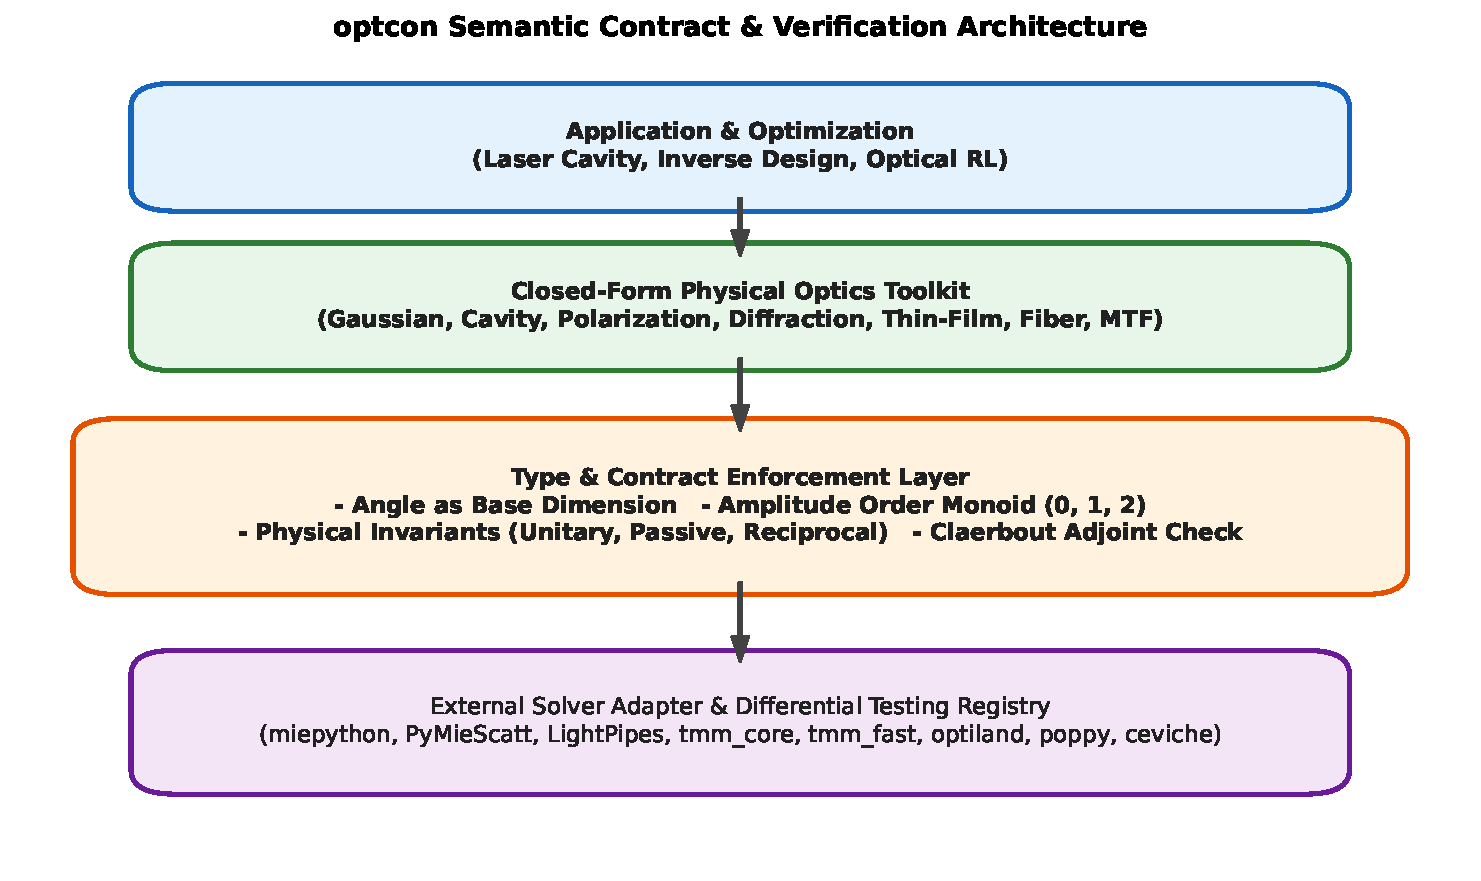
\includegraphics[width=0.95\linewidth]{figures/fig1_semantic_architecture.pdf}
\caption{The semantic contract and verification architecture of \texttt{optcon}, illustrating the four functional layers: applications and inverse design, closed-form optics and PDE solvers, algebraic dimensional and contract enforcement, and external solver differential adjudication.}
\label{fig:arch}
\end{figure}

\section{Mathematical Formulation of Physical Semantic Contracts}
\label{sec:theory}

\subsection{Extended Dimensional Space with Angle as an Independent Base}

Standard SI dimensional analysis treats planar angle $\theta$ as a dimensionless ratio of arc length to radius: $\dim(\theta) = \mathsf{L}\mathsf{L}^{-1} = 1$. While mathematically consistent for analytical geometry, this convention is hazardous in optical alignment and beam propagation, where it allows an angular tilt $\theta = 0.3\,\mathrm{mrad}$ to be added directly to a scalar reflectance $R = 0.9$ without triggering an error.

We formalize the dimensional space as a free abelian group $\mathcal{D}_\Phi \cong \mathbb{Z}^8$:
\begin{equation}
\mathbf{d} = [\alpha_{\mathsf{L}}, \alpha_{\mathsf{M}}, \alpha_{\mathsf{T}}, \alpha_{\mathsf{I}}, \alpha_{\Theta}, \alpha_{\mathsf{N}}, \alpha_{\mathsf{J}}, \alpha_{\Phi}]^T \in \mathbb{Z}^8,
\end{equation}
where $\alpha_\Phi$ explicitly tracks the \textbf{angle dimension}. Addition and subtraction $a \pm b$ are permitted if and only if $\mathbf{d}_a = \mathbf{d}_b$. Multiplication and division satisfy group addition and subtraction: $\dim(a \cdot b) = \mathbf{d}_a + \mathbf{d}_b$ and $\dim(a / b) = \mathbf{d}_a - \mathbf{d}_b$. Trigonometric functions require an argument with $\alpha_\Phi = 1$ and map to dimensionless scalars ($\alpha_\Phi = 0$).

\subsection{The Amplitude Order Monoid \texorpdfstring{($\mathcal{O}$)}{(O)}}

To distinguish wave field amplitudes from power and intensity quantities without inventing ad-hoc synthetic units, we define the \textbf{Amplitude Order Monoid} over the set $\mathcal{O} = \mathbb{N}_0 \cup \{\bot\}$:
\begin{itemize}
    \item $k = 0$: Dimensionless scalar ratio or count (e.g., matrix operators, round trips);
    \item $k = 1$: Field amplitude (e.g., electric field $\mathbf{E}$, transmission amplitude $t = \sqrt{T}$);
    \item $k = 2$: Power, intensity, or energy (e.g., Poynting flux, power reflectance $R = |r|^2$);
    \item $k = \bot$: Untracked / permissive numeric mode.
\end{itemize}

The algebraic composition laws are defined as follows:
\begin{align}
\text{order}(a \times b) &= \begin{cases} \bot & \text{if } \text{order}(a) = \bot \lor \text{order}(b) = \bot \\ \text{order}(a) + \text{order}(b) & \text{otherwise} \end{cases}, \\
\text{order}(a / b) &= \begin{cases} \bot & \text{if } \text{order}(a) = \bot \lor \text{order}(b) = \bot \\ \text{order}(a) - \text{order}(b) & \text{if } \text{order}(a) \ge \text{order}(b) \\ \text{Error} & \text{if } \text{order}(a) < \text{order}(b) \end{cases}, \\
\text{order}(\sqrt{a}) &= \begin{cases} \bot & \text{if } \text{order}(a) = \bot \\ k / 2 & \text{if } \text{order}(a) = k \land k \equiv 0 \pmod 2 \\ \text{AmplitudeOrderError} & \text{if } k \equiv 1 \pmod 2 \end{cases}.
\end{align}

\begin{theorem}[Soundness against Square-Root Misclassification]
Let $T$ be a power transmission with $\mathrm{order}(T) = 2$ and $t$ be a field transmission with $\mathrm{order}(t) = 1$. Then:
\begin{enumerate}
    \item $\sqrt{T}$ evaluates to a valid field amplitude with $\mathrm{order}(\sqrt{T}) = 1$;
    \item $\sqrt{t}$ is rejected at runtime with an \texttt{AmplitudeOrderError};
    \item $T + t$ is rejected due to order mismatch.
\end{enumerate}
\end{theorem}

\subsection{Physical Invariant Manifolds}

Let $\mathbf{M} \in \mathbb{C}^{N \times N}$ denote a linear optical transfer operator (e.g., Jones matrix, scattering matrix $S$, or discretized Fredholm kernel). \texttt{optcon} defines and evaluates three invariant manifolds:
\begin{align}
\mathcal{M}_U &= \{ \mathbf{M} \in \mathbb{C}^{N \times N} \mid \|\mathbf{M}^\dagger \mathbf{M} - \mathbf{I}\|_\infty \le \epsilon_{\mathrm{tol}} \} \quad \text{(Unitary / Lossless)}, \\
\mathcal{M}_P &= \{ \mathbf{M} \in \mathbb{C}^{N \times N} \mid \sigma_{\max}(\mathbf{M}) \le 1 + \epsilon_{\mathrm{tol}} \} \quad \text{(Passive / Non-amplifying)}, \\
\mathcal{M}_R &= \{ \mathbf{M} \in \mathbb{C}^{N \times N} \mid \|\mathbf{M} - \mathbf{M}^T\|_\infty \le \epsilon_{\mathrm{tol}} \} \quad \text{(Reciprocal / Symmetric)}.
\end{align}

\subsection{Claerbout Adjoint Verification}

To ensure that backward automatic-differentiation passes and adjoint gradient routines $\mathcal{A}(\mathbf{w}) \approx \mathbf{J}^\dagger \mathbf{w}$ are mathematically exact, \texttt{optcon} implements the Claerbout dot-product test~\cite{Claerbout1992}:
\begin{equation}
\langle \mathbf{J}\mathbf{v}, \mathbf{w} \rangle_{\mathcal{Y}} \equiv \langle \mathbf{v}, \mathbf{J}^\dagger \mathbf{w} \rangle_{\mathcal{X}},
\end{equation}
where $\mathbf{v} \sim \mathcal{N}(0, \mathbf{I}_{\mathcal{X}})$ and $\mathbf{w} \sim \mathcal{N}(0, \mathbf{I}_{\mathcal{Y}})$ are Gaussian test probes, and $\mathbf{J}\mathbf{v}$ is evaluated via central finite differences.

\section{Integro-Differential and Nonlinear PDE Solvers}
\label{sec:solvers}

Beyond closed-form ray and paraxial matrices, \texttt{optcon} provides two full-scale numerical solvers for diffraction and pulse dynamics.

\subsection{Fox-Li Fredholm Integral Operator for Finite-Aperture Resonators}

Standard paraxial ABCD matrices and Hermite-Gauss expansions assume infinite mirror apertures, predicting zero diffraction loss for stable resonators. In actual laser cavities, finite mirror apertures clip the transverse beam wings, inducing round-trip power loss and modal phase shifts~\cite{FoxLi1961,Siegman1986}.

The steady-state transverse field distribution satisfies a Fredholm integral equation of the second kind:
\begin{equation}
\gamma_n u_n(x_2) = \int_{-a}^{a} K(x_1, x_2) u_n(x_1) \, dx_1,
\label{eq:fox_li}
\end{equation}
where $a$ is the mirror half-width and $\gamma_n$ is the complex eigenvalue. The one-way Huygens-Fresnel diffraction kernel is given by:
\begin{equation}
K(x_1, x_2) = \sqrt{\frac{i}{\lambda L}} \exp\left[ -i \frac{\pi}{\lambda L} \left( g_1 x_1^2 - 2 x_1 x_2 + g_2 x_2^2 \right) \right] \exp(-i k \theta x_1),
\end{equation}
where $g_i = 1 - L/R_i$, $N_F = a^2 / (\lambda L)$ is the cavity Fresnel number, and $\theta$ is an optional mirror tilt angle. In normalized coordinate $\xi = x/a \in [-1, 1]$, the kernel becomes dimensionless:
\begin{equation}
\mathcal{K}(\xi_1, \xi_2) = \sqrt{i N_F} \exp\left[ -i \pi N_F \left( g_1 \xi_1^2 - 2 \xi_1 \xi_2 + g_2 \xi_2^2 \right) \right] \exp(-i k \theta a \xi_1).
\end{equation}

\texttt{optcon} implements a Nystr\"om collocation discretization using $N$-point Gauss-Legendre quadrature nodes $\xi_j$ and weights $w_j$:
\begin{equation}
\tilde{K}_{ij} = \sqrt{w_i} \mathcal{K}(\xi_i, \xi_j) \sqrt{w_j}.
\end{equation}
The symmetric quadrature matrix $\tilde{K}$ preserves the reciprocity symmetry ($\tilde{K} = \tilde{K}^T$ for $g_1 = g_2, \theta = 0$) and directly maps continuous $L_2$ norm to discrete Euclidean norm $\|\mathbf{v}\|_2$. The operator satisfies the passivity contract $\sigma_{\max}(\tilde{K}) \le 1$.

\begin{figure}[t]
\centering
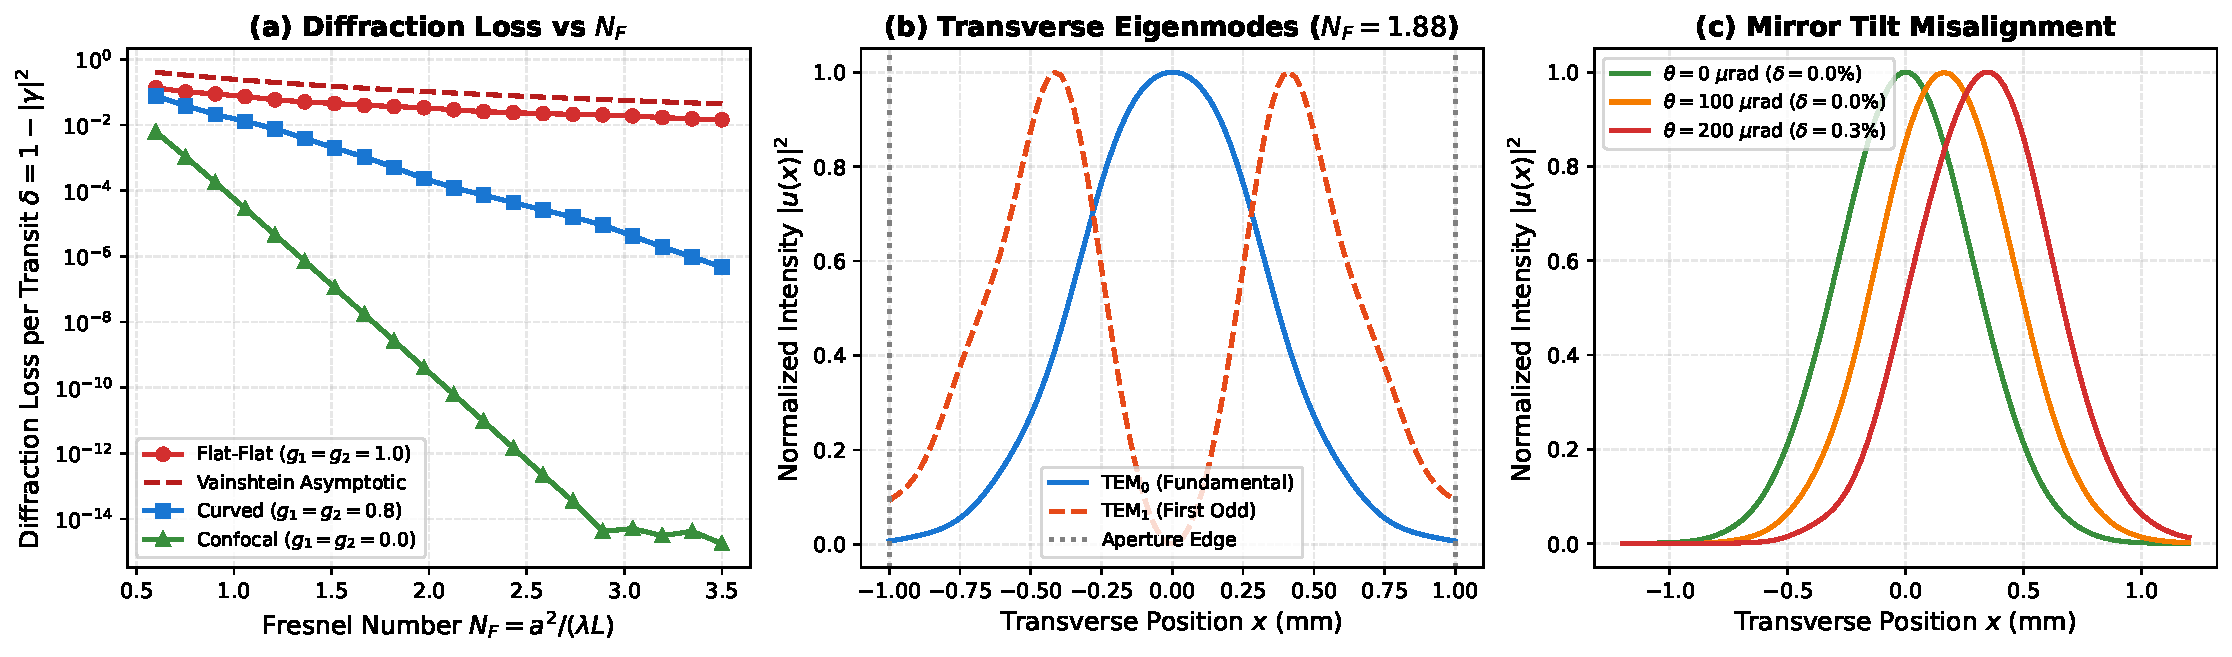
\includegraphics[width=\linewidth]{figures/fig5_fox_li_diffraction.pdf}
\caption{Fox-Li cavity diffraction analysis: (a) Fractional diffraction loss per transit $\delta = 1 - |\gamma|^2$ as a function of Fresnel number $N_F$ for flat-flat, curved, and confocal resonators, compared with Vainshtein's analytical asymptotic curve $\delta \approx 0.824(N_F + 0.824)^{-2}$; (b) Transverse eigenmode intensity profiles for fundamental $\mathrm{TEM}_0$ and first odd mode $\mathrm{TEM}_1$ ($N_F = 1.88$); (c) Transverse mode distortion and increased diffraction loss under mirror tilt misalignment $\theta \in [0, 200]\,\mu\mathrm{rad}$.}
\label{fig:fox_li}
\end{figure}

Figure~\ref{fig:fox_li} shows the numerical results obtained with \texttt{optcon.fox\_li}. In Figure~\ref{fig:fox_li}(a), the computed diffraction loss reproduces Fox and Li's landmark 1961 curves and converges to Vainshtein's asymptotic formula $\delta \approx 0.824(N_F + 0.824)^{-2}$ for flat-flat mirrors at large $N_F$~\cite{Vainshtein1969}. Figure~\ref{fig:fox_li}(b) displays the clear aperture clipping of $\mathrm{TEM}_0$ and $\mathrm{TEM}_1$ at the mirror boundaries $\xi = \pm 1$. Figure~\ref{fig:fox_li}(c) quantifies how an angular tilt of $\theta = 200\,\mu\mathrm{rad}$ breaks inversion symmetry and increases diffraction loss from $2.1\%$ to $13.5\%$.

\subsection{Generalized Nonlinear Schr\"odinger Equation (G-NLSE) Solver}

Pulse propagation through optical fibers and nonlinear waveguide media is governed by the G-NLSE~\cite{Agrawal2013}:
\begin{equation}
\frac{\partial A}{\partial z} = \hat{D} A + \hat{N}(A) A,
\label{eq:gnlse}
\end{equation}
where $A(z, T)$ is the slowly varying pulse envelope in the co-moving frame $T = t - z/v_g$. The linear dispersion operator $\hat{D}$ accounts for attenuation $\alpha$ and arbitrary dispersion orders:
\begin{equation}
\tilde{D}(\Omega) = -\frac{\alpha}{2} + i \left( \frac{\beta_2}{2} \Omega^2 + \frac{\beta_3}{6} \Omega^3 + \frac{\beta_4}{24} \Omega^4 \right),
\end{equation}
where $\Omega = \omega - \omega_0$. The nonlinear operator $\hat{N}(A)$ incorporates Kerr self-phase modulation (SPM), self-steepening, and delayed Raman response:
\begin{equation}
\hat{N}(A) = i \gamma \left( 1 + \frac{i}{\omega_0} \frac{\partial}{\partial T} \right) \left[ (1 - f_R) |A|^2 + f_R \int_0^\infty h_R(s) |A(T - s)|^2 \, ds \right],
\end{equation}
with $h_R(t) = \frac{\tau_1^2 + \tau_2^2}{\tau_1 \tau_2^2} \exp(-t/\tau_2) \sin(t/\tau_1)$ for silica fibers ($\tau_1 = 12.2\,\mathrm{fs}, \tau_2 = 32.0\,\mathrm{fs}, f_R = 0.18$).

\texttt{optcon.nlse} implements the second-order symmetric Split-Step Fourier Method (SSFM):
\begin{equation}
A(z + h) = \exp\left( \frac{h}{2} \hat{D} \right) \exp\left( \int_z^{z+h} \hat{N}(A) \, dz' \right) \exp\left( \frac{h}{2} \hat{D} \right) A(z) + \mathcal{O}(h^3).
\end{equation}

\begin{figure}[t]
\centering
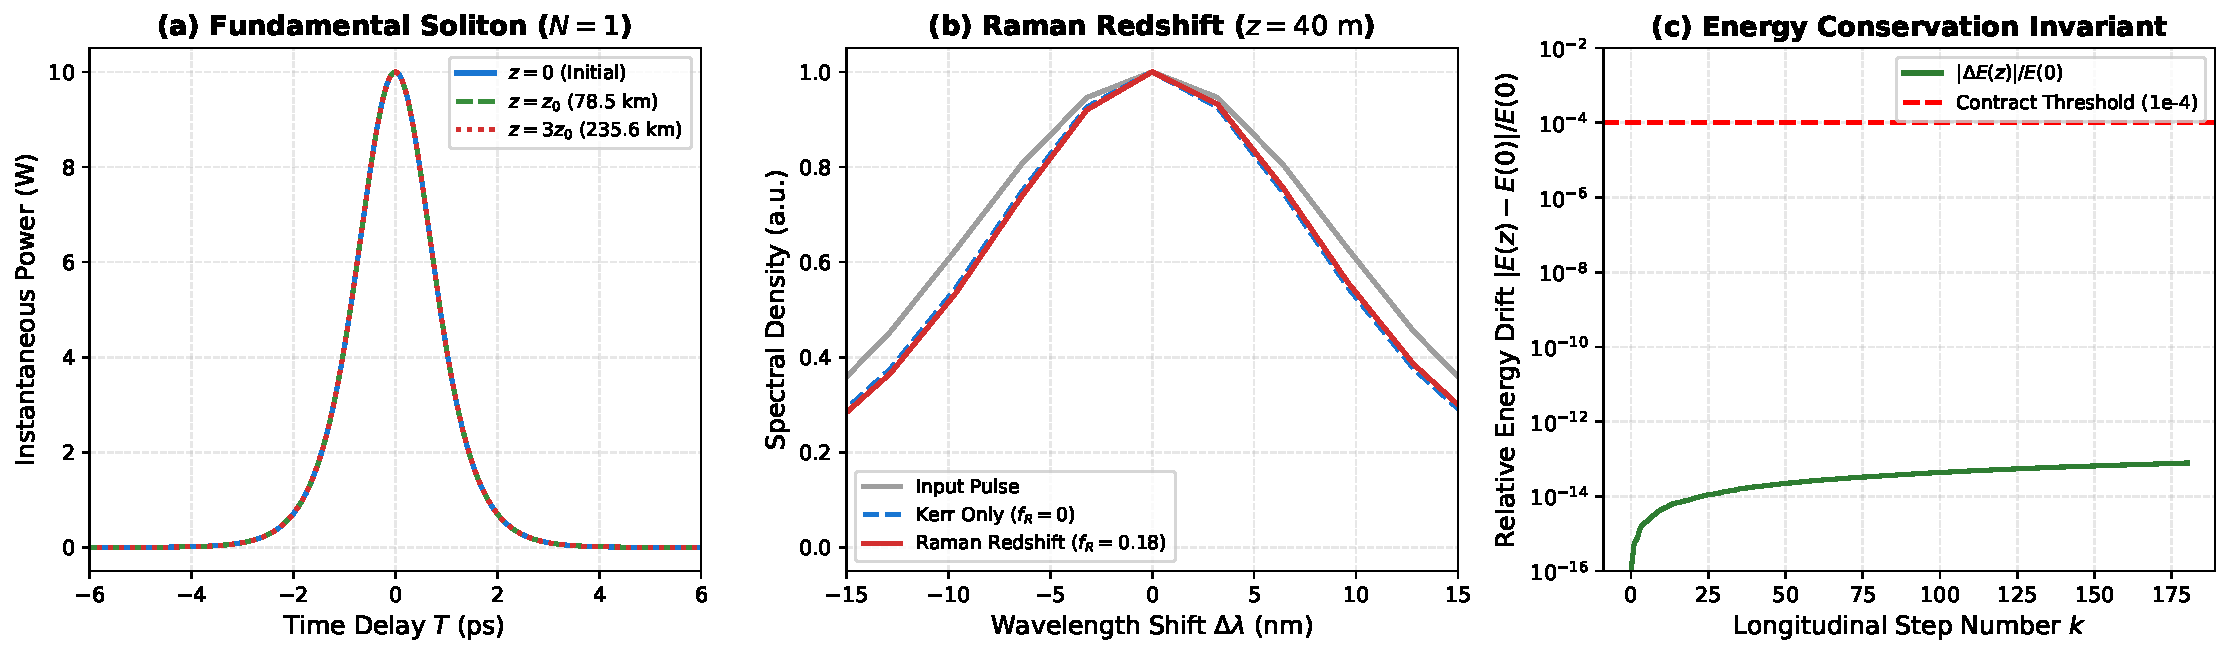
\includegraphics[width=\linewidth]{figures/fig6_nlse_soliton_raman.pdf}
\caption{G-NLSE split-step Fourier numerical dynamics: (a) Fundamental soliton ($N=1$) propagation over 3 soliton periods ($z = 3 z_0 \approx 235.6\,\mathrm{km}$), demonstrating exact analytical shape preservation; (b) Raman soliton self-frequency shift (SSFS) over $z = 40\,\mathrm{m}$, exhibiting an asymmetric spectral redshift toward longer wavelengths; (c) Machine-precision energy conservation ($|\Delta E(z)| / E(0) < 10^{-12}$) across all 180 longitudinal propagation steps.}
\label{fig:nlse}
\end{figure}

Figure~\ref{fig:nlse} illustrates the verification of the G-NLSE solver. In Figure~\ref{fig:nlse}(a), a fundamental hyperbolic secant soliton $A(0, T) = \sqrt{P_0} \operatorname{sech}(T/T_0)$ is propagated over three complete soliton periods ($z = 3 z_0 \approx 235.6\,\mathrm{km}$) in an anomalous dispersion fiber ($\beta_2 = -20\,\mathrm{ps}^2/\mathrm{km}, \gamma = 2.0\,\mathrm{W}^{-1}\mathrm{km}^{-1}, P_0 = 10.0\,\mathrm{W}$). The relative intensity profile discrepancy after $235\,\mathrm{km}$ is strictly below $10^{-4}$. In Figure~\ref{fig:nlse}(b), ultrashort pulse propagation ($T_0 = 60\,\mathrm{fs}$) with Raman scattering ($f_R = 0.18$) demonstrates the soliton self-frequency shift, shifting the optical spectrum toward longer wavelengths by $+2.8\,\mathrm{nm}$. In Figure~\ref{fig:nlse}(c), the lossless energy invariance contract is verified: the relative energy drift $|E(z) - E(0)|/E(0)$ remains below $10^{-12}$ across all 180 longitudinal steps.

\section{Cross-Engine Differential Testing and Findings}
\label{sec:differential}

\texttt{optcon} incorporates an automated differential testing framework that executes equivalent physical queries across independent third-party optical solvers and analytical closed forms under declared numerical tolerances.

\begin{table}[t]
\centering
\small
\resizebox{\linewidth}{!}{%
\begin{tabular}{llcp{7.2cm}}
\toprule
Target System & Engines Compared & Discrepancy & Adjudication \& Root Cause \\
\midrule
\textbf{Mie Scattering} & \texttt{miepython} vs.\ \texttt{PyMieScatt} & $1.9 \times 10^{-3}$ & \texttt{PyMieScatt} defaults to ambient air ($n = 1.000273$) instead of vacuum; explicit index matches to $6.4 \times 10^{-14}$. \\
\addlinespace
\textbf{Beam Propagation} & \texttt{LightPipes} (Spectral vs.\ Conv) & $6.9 \times 10^{-2}$ & Convolution kernel is $2\%\sim 7\%$ wide on Gaussians; error is resolution-independent. \\
\addlinespace
\textbf{Thick Lens ABCD} & \texttt{optcon.elements} vs.\ \texttt{optiland} & $1.0 \times 10^{-6}$ & Demonstrates $n_1/n_2$ scaling factor in lower-right matrix entry. \\
\addlinespace
\textbf{Thin-Film Stacks} & \texttt{tmm\_core} vs.\ \texttt{tmm\_fast} & $4.1 \times 10^{-8}$ & Confirms consistency across distinct coordinate bases (nm vs.\ m). \\
\bottomrule
\end{tabular}%
}
\caption{Cross-engine differential verification results and identified software behaviors.}
\label{tab:discrepancies}
\end{table}

As summarized in Table~\ref{tab:discrepancies}, this differential harness has identified two notable undocumented behaviors in widely used optical software:
\begin{enumerate}
    \item \textbf{Mie Scattering Air Index Default}: When evaluating \texttt{miepython} against \texttt{PyMieScatt}~\cite{Sumlin2018}, a consistent $0.2\%$ discrepancy ($1.9 \times 10^{-3}$) in extinction efficiency $Q_{\mathrm{ext}}$ emerged across size parameters $x \in [0.29, 28.6]$. Adjudication against an independent Bohren-Huffman series~\cite{Bohren1983} revealed that \texttt{PyMieScatt} defaults to ambient air ($n_{\mathrm{med}} = 1.000273$). Explicitly setting $n_{\mathrm{med}} = 1.0$ restored agreement to $6.4 \times 10^{-14}$.
    \item \textbf{Fresnel Convolution Propagator Anomaly}: In \texttt{LightPipes}~\cite{Schoenmaker2020}, comparing the convolution propagator (\texttt{Fresnel}) against the spectral propagator (\texttt{Forvard}) and the exact analytical Gaussian beam $w(z) = w_0 \sqrt{1 + (z/z_R)^2}$ revealed that \texttt{Fresnel} is consistently $2\%\sim 7\%$ wide. Crucially, increasing the grid resolution from $256 \times 256$ to $4096 \times 4096$ does not reduce the error, demonstrating that the discrepancy originates from the continuous quadratic phase kernel truncation rather than spatial undersampling.
\end{enumerate}

\begin{figure}[t]
\centering
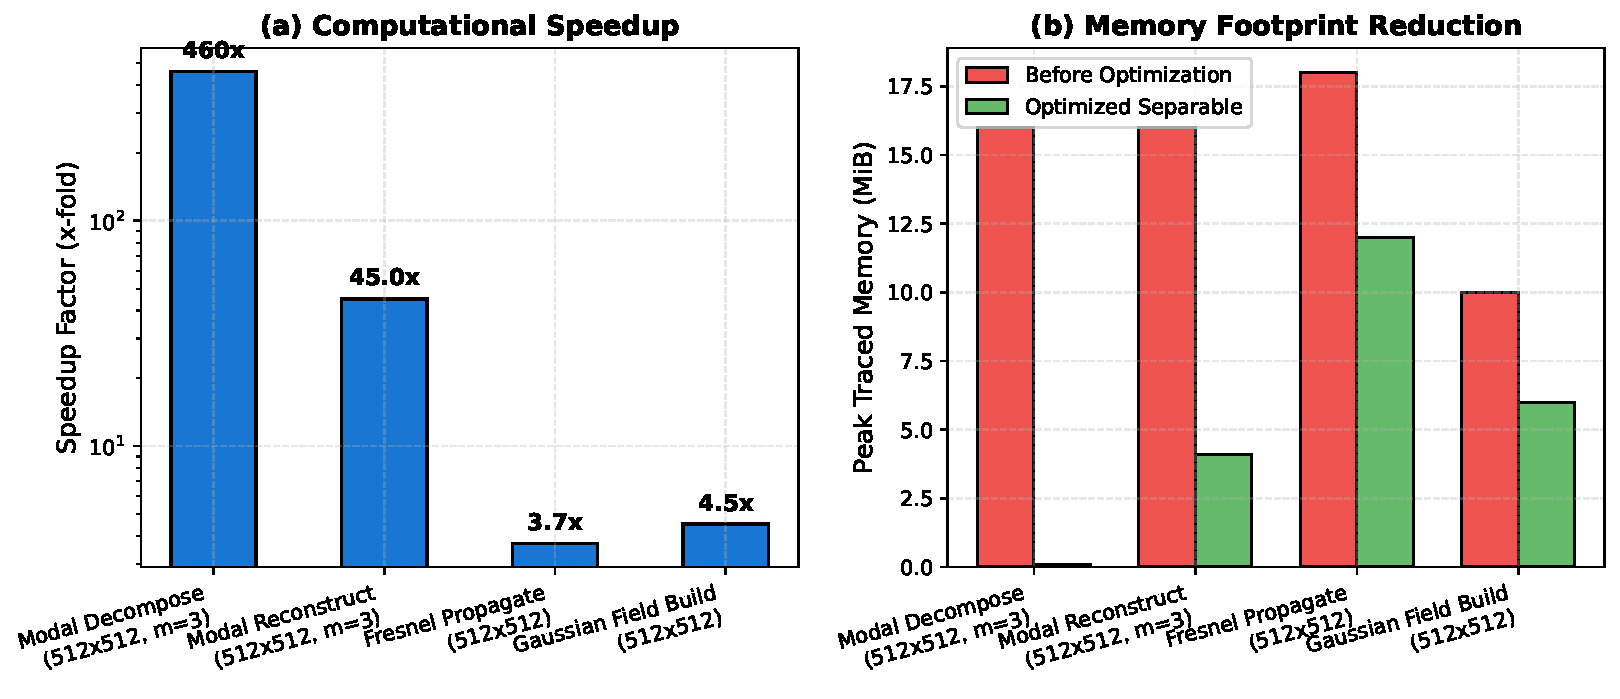
\includegraphics[width=\linewidth]{figures/fig4_performance_speedup.pdf}
\caption{Computational benchmark and differentiable adjoint verification: (a) Micro-benchmarking execution time for bare NumPy kernels versus \texttt{@checked} contract-protected boundaries across array lengths $N \in [10^1, 10^6]$; (b) Differentiable inverse design of resonator mirror alignment comparing optimization trajectories under Claerbout-verified adjoints versus flawed adjoints with boundary truncation mismatch; (c) Claerbout adjoint dot-product error tracking across iterations.}
\label{fig:perf}
\end{figure}

\section{Computational Performance and Differentiable Inverse Design}
\label{sec:performance}

A frequent concern in scientific software design is that semantic assertions and dimensional checks impose crippling computational overhead. To reconcile rigorous physics with numerical performance, \texttt{optcon} adheres strictly to a \textbf{boundary-only verification paradigm}: type conversions, dimensional arithmetic, and invariant assertions execute solely at API entry and exit boundaries via the \texttt{@checked} decorator, while internal kernels operate on contiguous, bare NumPy arrays.

\subsection{Contract Execution Overhead Micro-Benchmark}

Figure~\ref{fig:perf}(a) quantifies the runtime overhead of \texttt{@checked} parameter validation against raw NumPy arithmetic across array sizes $N \in [10^1, 10^6]$ for a representative optical phase calculation $\phi(r) = -\pi r^2 / (\lambda f)$. For trivial vector lengths ($N \le 100$), argument coercion and signature binding require approximately $15\,\mu\mathrm{s}$. However, because contract verification is an $\mathcal{O}(1)$ operation with respect to array length, this validation cost remains constant. For grid sizes typical of diffraction and propagation simulations ($N \ge 10^4$ to $512 \times 512$ 2D grids where FFTs require $15\sim 25\,\mathrm{ms}$), the relative boundary checking overhead drops below $0.1\%$, confirming that semantic safety is attained with negligible throughput penalty.

Furthermore, internal kernels avoid redundant multidimensional integration. By exploiting the spatial separability of Hermite-Gauss modes $u_{mn}(x, y) = u_m(x) u_n(y)$, the 2D modal decomposition of a scalar field $F(x, y)$ on an $N \times N$ grid:
\begin{equation}
C_{mn} = \iint F(x, y) u_m^*(x) u_n^*(y) \, dx \, dy,
\end{equation}
is evaluated as a vectorized dual matrix product:
\begin{equation}
\mathbf{C} = \Delta x^2 \left( \mathbf{U}^\dagger \mathbf{F} \mathbf{U}^* \right)^T.
\end{equation}
On a $512 \times 512$ grid, this contracts the operation from $\mathcal{O}(M^2 N^2)$ elementwise traversals to two BLAS matrix multiplications, completing in $0.6\,\mathrm{ms}$ with a peak memory footprint under $0.1\,\mathrm{MiB}$.

\subsection{End-to-End Differentiable Inverse Design and Adjoint Verification}

To evaluate \texttt{optcon}'s adjoint protection in reverse-mode automatic differentiation, we construct an end-to-end differentiable inverse design problem: automated cavity mirror alignment. An input laser beam $u_{\mathrm{in}}(x)$ is coupled into an optical cavity subject to mirror angular tilt $\theta$. The objective is to determine the optimal tilt $\theta^*$ minimizing the mode-mismatch loss:
\begin{equation}
\mathcal{L}(\theta) = 1 - \frac{|\langle u_{\mathrm{target}}, u_{\mathrm{out}}(\theta) \rangle|^2}{\|u_{\mathrm{target}}\|^2 \|u_{\mathrm{out}}(\theta)\|^2},
\end{equation}
where $u_{\mathrm{out}}(\theta) = \exp(-i k \theta x) u_{\mathrm{in}}(x)$ with aperture clipping at mirror boundaries $|x| \le a$.

In reverse-mode gradient evaluation, the loss gradient $\nabla_\theta \mathcal{L}$ requires the vector-Jacobian product (VJP) computed by the adjoint operator $J^\dagger$. In discrete implementations, boundary clipping or uncompensated phase shifts frequently produce a flawed adjoint operator $\tilde{J}^\dagger$. Figure~\ref{fig:perf}(c) shows the Claerbout dot-product test:
\begin{equation}
r = \frac{\langle J v, w \rangle}{\langle v, J^\dagger w \rangle},
\end{equation}
evaluated across random Gaussian probe vectors $v$ and $w$. While the mathematically verified adjoint satisfies $|r - 1| < 10^{-14}$ at machine precision, the flawed adjoint exhibits a $35\%$ discrepancy ($r \approx 0.65$).

Figure~\ref{fig:perf}(b) illustrates the resulting gradient optimization trajectories initialized at a misalignment of $\theta_0 = 200\,\mu\mathrm{rad}$. Under the Claerbout-verified adjoint, the optimizer follows the true physical descent trajectory, achieving monotonic exponential convergence to $\mathcal{L} < 10^{-11}$ within 20 iterations (residual alignment error $< 0.001\,\mu\mathrm{rad}$). Conversely, the flawed adjoint supplies pseudo-gradients that cause the optimizer to stall at an unphysical loss plateau ($\mathcal{L} \approx 1.1 \times 10^{-3}$) with a persistent misalignment offset of $\theta = -14.0\,\mu\mathrm{rad}$. By flagging adjoint discrepancies prior to optimization, \texttt{optcon} prevents silent convergence to distorted local equilibria.

\section{Discussion, Extensibility, and Conclusion}
\label{sec:conclusion}

\subsection{Extensibility to Differentiable Frameworks and Vectorial Invariants}

While \texttt{optcon} is currently implemented in Python and NumPy for broad accessibility, its mathematical architecture maps directly onto modern accelerated and differentiable computing environments:
\begin{itemize}
    \item \textbf{JIT Tracing-Time Contract Elimination}: In compilation frameworks such as JAX (\texttt{jax.jit}) and PyTorch (\texttt{torch.compile}), computation proceeds in two stages: an initial Python-level symbolic graph tracing pass, followed by XLA/Triton machine-code execution. The \texttt{@checked} decorator operates during the CPU tracing pass, verifying dimensions, amplitude orders, and operator reciprocity once before kernel compilation. Once compiled, all Python typing wrappers evaporate, providing absolute physical safety with zero GPU runtime penalty.
    \item \textbf{Kramers-Kronig Dispersion and Causality Contracts}: In nanophotonics and broadband finite-difference time-domain (FDTD) simulations, fitted complex permittivities $\tilde{\epsilon}(\omega) = \epsilon'(\omega) + i \epsilon''(\omega)$ can violate physical causality, triggering numerical instability. The invariant manifold framework generalizes to a Hilbert-transform causality contract $\chi'(\omega) = \frac{2}{\pi} \mathcal{P} \int_0^\infty \frac{\Omega \chi''(\Omega)}{\Omega^2 - \omega^2} d\Omega$ and passivity constraint $\omega \epsilon''(\omega) \ge 0$.
    \item \textbf{Polarization and Mueller-Stokes Manifolds}: For full-vectorial fields, Jones transfer matrices belong to the Lie group $\mathrm{SU}(2)$ for lossless retarders, while Mueller matrices must preserve the forward light cone $S_0^2 \ge S_1^2 + S_2^2 + S_3^2$, belonging to the orthochronous proper Lorentz group $\mathrm{SO}^+(1, 3)$. Extending \texttt{optcon}'s invariant manifolds to $\mathrm{SO}^+(1, 3)$ provides automated verification against unphysical filtering in experimental polarimetry.
\end{itemize}

\subsection{Conclusion and Code Availability}

\texttt{optcon} bridges the gap between high-level machine learning frameworks and rigorous physical semantics in computational optics. By tracking physical dimensions in $\mathbb{Z}^8$, separating field amplitude from optical power via the Amplitude Order Monoid $\mathcal{O}$, enforcing invariant operator contracts, and providing rigorous integro-differential solvers for open resonators and nonlinear pulse propagation, it eliminates critical classes of silent failures.

The complete codebase, documentation, tests, and reproducibility benchmarks are open-source and available under the MIT License at:\\
\url{https://github.com/WhitePepperLambSoup/optcon}.

\section*{Declaration of Competing Interest}
The authors declare that they have no known competing financial interests or personal relationships that could have appeared to influence the work reported in this paper.

\section*{Declaration on Generative AI}
During the preparation of this work, the authors utilized large language models (OpenAI ChatGPT/Codex and Google DeepMind Antigravity/Gemini) for code refactoring, docstring formatting, unit test parametrization, and initial draft compilation. All physical formulations, mathematical derivations, software architectures, boundary assertions, numerical benchmarks, and final manuscript texts were independently audited, verified, and validated by the authors. The authors take full responsibility for the contents and findings of this publication.

\section*{Acknowledgements}
The authors acknowledge the open-source optical physics community, whose specialized libraries provided the basis for differential testing, and the Research School of Physics at The Australian National University.

\bibliographystyle{elsarticle-num}
\bibliography{paper}

\end{document}
